\chapter{Popis jadra cortex M3}
\section{Úvod}


Prvé mikroprocesory úspešne napredovali vo zvyšovaní výkonu vďaka zvyšovaniu počtu inštrukcií a zvyšovaniu taktovacej frekvencie. V 80-tych rokoch sa však ukázalo, že to nie je najlepšia cesta - dekóder inštrukcií mikroprocesora bol so vzrastajúcim počtom inštrukcií čoraz zložitejší a nastávali aj problémy so zreťazením inštruckií, či predikciou skokov. Páni Steve Furber a Sophie Wilson \cite{root_arm} si po preštudovaní dostupných publikácií a dôkladnej analýze uvedomili silné možnosti architektúry RISC 1, ktorá ponúkala pozoruhodný výpočtový výkon len so 44000 tranzistormi a 31 inštrukciami. Kľúčovou myšlienkou bol fakt, že ani programátor, ani kompilátor nedokážu optimálne využiť komplexné sady inštrukcií. 

Ich práca a vznik firmy Acorn vydláždili cestu k architektúre ARM 1. Prvé ARM jadro malo troj stupňové zreťazenie - načítanie, dekódovanie a vykonanie inštrukcie bolo v idéalnom prípade vykonávané pre tri inštrukcie naraz, každá v inom štádiu. Problém predstavovali a do dnes predstavujú inštrukcie podmienených skokov. Redukovaním počtu inštrukcií a prístupom do pamäte len pomocou inštrukcií load store tento neduh veľmi dobre redukuje. Ďalším prínosom ARM 1 jadra bol veľký počet registrov (pôvodne 37), všetky sú rovnocenné a dokonca programový čítač je namapovaný k týmto registrom, čo opäť umožňuje znížiť počet inštrukcií. Túto techniku využíva aj jadro msp430 \cite{msp430_mcu} .

Netrvalo dlho a vývojári si osvojili výhody jadra ARM. Dnes je známych mnoho verzií. Pre ilustráciu sú to napríklad popuĺárne ARM7TDMI, ARM11, ARM Cortex M, ARM Cortex R a veľmi výkonná rada ARM Cortex A \cite{arm_list} . Séria jadier Cortex A je populárna najmä v aplikačnej oblasti : inteligentné telefóny, tablety, dvd a blue ray prehrávače. Dá sa očakávať ich postupné nasadenie v osobných počtačoch. Výhodou je najmä spotreba a cena, ktorú znižuje nadol silná konkurencia.

Práca je zameraná na jadro Cortex m3 a Cortex m4. Je to rada so širokým spektrom použitia, najmä pre priemyselné aplikácie, aplikácie s nízkou spotrebou a citlivé na cenu. Najlepším príkladom ich porovnania, z pohľadu inštrukčnej sady je nasledujúci obrázok.

\begin{figure}[ht]
\begin{center}
\begin{minipage}{1.1\linewidth}
\begin{center}
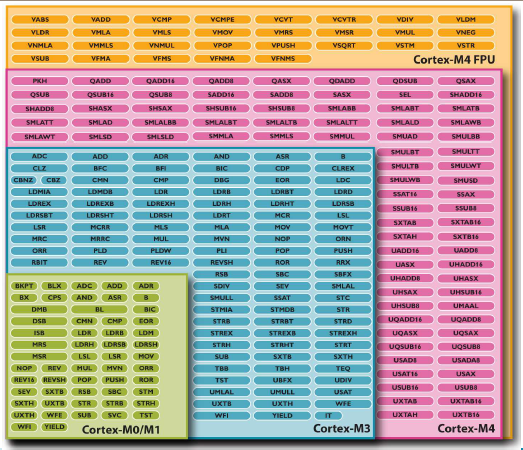
\includegraphics[width=.8\textwidth]{images/cm_instructions.png}
\caption{Porovnanie jadier Cortex Mx }
\label{obr1}
\end{center}
\end{minipage}
\end{center}
\end{figure}

Z obrázku je zrejmé, že jadrá sú navzájom kompatibilné, smerom k nižším modelom. Z konkrétnych typov mikrokontrolérov boli zvolené stm32f100 a lm4f120. Najmä pre ich bezproblémovú dostupnosť a cenu. Ako programátor pre stm32 bola použitá doska stm32 discovery kit a pre lm4f120 doska stellaris launchpad. Cena oboch dosiek je vzhľadom na možnosti použitia veľmi nízka (pod 15eur). S doskami je možné programovať aj mikrokontroléry v externej aplikácií, stačí počítač s USB rozhraním.

Pre samotné pochopenie a analýzu operačného systému je ale treba najprv rozobrať ich vnútornú, najmä registrovú štruktúru a princip funkcie radiča prerušení.

\section{Popis registrov}

Pre správnu funkciu mikroprocesora stačí minimum registrov : programový čítač, stavový register a register práve vykonávanej inštrukcie. Takto bolo navrhnuté jadro 68HC11 \cite{68HC11}. Obsahuje len dva univerzálne registre A, B, ukazovateľové registre X, Y a programový čítač spolu s ukazovateľom na zásobník. Snaha bola využiť dostupnú pamäť ako priestor na usutočňovanie všetkých operácií. Pre zvýšenie výpočtového výkonu, to však bola nesprávna cesta. Mikroprocesor musel takmer vždy vyberať operandy z pamäte a tieto operácie zaberú viac času, ako prístup do registrov. Jadro ARM preto zvolilo cestu vysokého počtu registrov. Problém nízkeho počtu registrov je aj v nemožnosti zreťazenia inštrukcií - inštrukcie je možné vykonávať paralelne len ak nie sú na sebe závislé (konflikt rovnakých registrov, alebo rovnaké adresy v pamäti).

Jadro ARM pre minimalizáciu počtu prístupov do pamäte využíva vysoký počet univerzálnych registrov. Registre R0 až R12 sú univerzálne použiteľné a dostupné pre aplikáciu. Register R13 je ukazovateľ zásobníka. Register R14 predstavuje tzv. Link register. Mikroprocesor doň ukladá návratovú adresu funkcie. Pri jednoúrovňových volaniach sa tak nemusí pristupovať na zásobník. Pre viacúrovňové volania sa už hodnota musí ukladať aj na zásobník, pričom posledne volaná funkcia má návratovú adresu vždy v LR registri. Programový čítač je prístupný ako register R15. Jadro je ďalej vybavené niekoľkými stavovými registrami, súhrnne označované ako xPSR. Tieto registre uchovávajú stav procesora a prerušení. Podrobnejší popis je možné nájsť v pekne spracovanej príručke Inside Cortex \cite{inside_cortex}

Inštrukčná sada ARM jadra plne využíva princíp load-store. Maximum operácií sa vykonáva medzi registrami. Nie je výnimkou použitie trojoperandových inštrukcií.  


\begin{figure}[ht]
\begin{center}
\begin{minipage}{1.1\linewidth}
\begin{center}
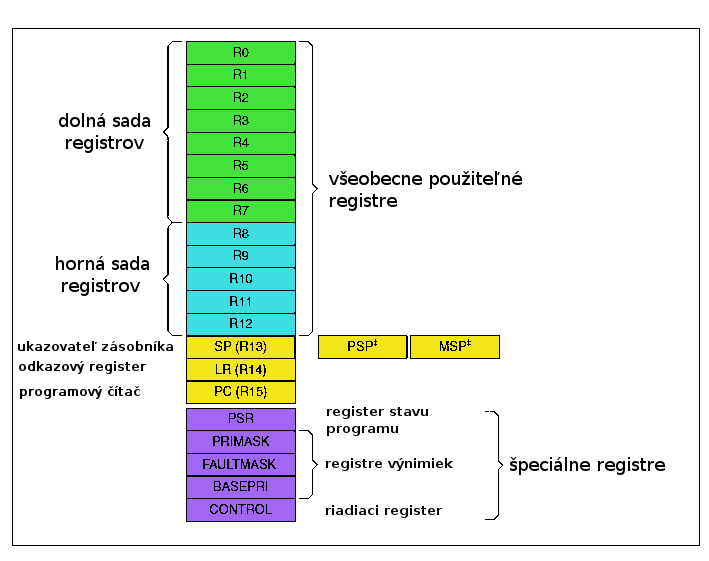
\includegraphics[width=.75\textwidth]{images/STM32F10xx_processor_core_registers.png}
\caption{Registre jadra Cortex M3 }
\label{obr2}
\end{center}
\end{minipage}
\end{center}
\end{figure}


\section{Jednotka NVIC}

Všetky mikrokontroléry s jadrom ARM Cortex sú vybavené pokročilou jednotkou správy prerušení. Jednotka NVIC je navrhnutá s ohľadom na minimalizáciu latencií prerušení. Taktiež zabezpečuje deterministickú obsluhu prerušení. Pre mikrokontrolér STM32F je k dispozícií 16 úrovní priorít prerušení.

Po hardvérovom generovaní prerušenia spustí NVIC sekvenciu niekoľkých krokov. Najprv sa dokončí práve vykonávaná inŠtrukcia. Následne sa pomocou mikrokódu uložia horné registre - nie je potrebný žiaden softvérovy zásah. Proces ukladania registrov trvá 12 hodinových cyklov. Následne sa spustí samotné vykonanie obsluhy prerušenia - užívateľská časť. Po ukončení vykonávania obsluhy sa opäť pomocou mikrokódu obnovia registre. Operácia obnovy taktiež trvá 12 cyklov.


\begin{figure}[ht]
\begin{center}
\begin{minipage}{1.1\linewidth}
\begin{center}
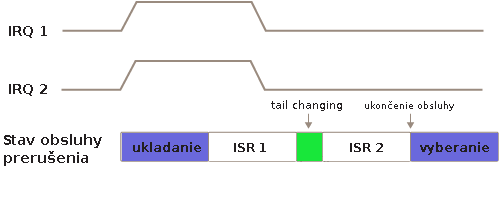
\includegraphics[width=.75\textwidth]{images/irq_sequence.png}
\caption{Sekvencia obsluhy prerušenia}
\label{obr2}
\end{center}
\end{minipage}
\end{center}
\end{figure}

Obrázok znázorňuje prioritný proces obsluhy dvoch prerušení. Prerušenie IRQ 1 má vyššiu prioritu. V krátkom okamihu nastanú požiadavky na obsluhu oboch prerušení. Jednotka NVIC uloží registre a spustí prvú obslužnú rutinu. Po jej ukončení sa vykoná tzv. tail changing - namiesto návratu do hlavnej slučky programu a opätovného ukladania registrov sa spustí obsluha druhého prerušenia. Táto operácia trvá len 6 strojových cyklov. Po dokončení obsluhy prerušenia sa obnovia registre a program pokračuje v hlavnej slučke.

Celkovo, sekvencia réžie trvá 30 strojových cyklov. Ak by nebola využitá možnosť tail changing, bolo by to 48 cyklov. Jednotka NVIC tak pomáha minimalizovať časové latencie a zjednodušiť návrh systému pracujúceho v reálnom čase.


\section{Tabuľka prerušení}

Prerušenie je reakcia na asynchronnú udalosť. Pôvodne bolo vyvinuté pre obsluhu pomalých periférií - procesor by bez prerušovacieho systému musel zbytočne čakať na dokončenie pomalej periférnej operácie. Vo svete programovania PC je možné sa stretnúť so softvérovými prerušeniami (int 10h, int 21h, int 80h). Názov je však zavádzajúci. V skutočnosti sa jedná o plne synchrónnu operáciu a je to volanie podprogramu uloženého na pevnej adrese.

Tabuľka prerušení jadra Cortex M3 má dve časti. V pamäti je však spojitá. Prvá časť sú vektory prerušení, spoločné pre všetky jadrá triedy Cortex M. Hneď za ňou sa nachádza druhá časť, ktorá obsahuje vektory závislé od použitých periférií. Nakoľko operačný systém má byť nezávislý od periférií, je z tohto pohľadu dôležitá len prvá časť. 

Treba poznamenať, že tabuľka musí byť uložená v sekcií isr\_vectors (nachádza sa obvykle na začiatku programovej pamäte). Prvá položka tabuľky je ukazovateľ na zásobník. Jadro podľa jej hodnoty nastavuje ukazovateľ zásobníka v RAM pamäti.


{\small
\begin{verbatim}
__attribute__ ((section(".isr_vector")))
void (* const g_pfnVectors[])(void) = {
					    // počiatočný stav zásobníka
    (void (*)(void))((unsigned long)pulStack + sizeof(pulStack)),
                                            
    ResetISR,                               // reset prerušenie
    NmiSR,                                  // NMI prerušenie
    FaultISR,                               // prerušenie kritického zlyhania
    ...
    SYS_TICK_INT,        	            // prerušenie systémového časovača
    ...
\end{verbatim}
}

Nasleduje položka \textbf{ResetISR}. To je vstupný bod do programu. Na tejto adrese začína mikrokontrolér vykonávať program. Táto funkcia obvykle predstavuje štartovaciu sekvenciu. Je však možné umiestniť sem ukazovateľ na funkciu main() a začať bez štartovacej sekvencie.

Z pohľadu stability systému je veľmi dobre využitá položka \textbf{FaultISR}. Toto prerušenie sa vyvolá pri vykonávaní nesprávnej alebo neoprávnenej inštrukcie. Odchytom tejto udalosti je možné emulovať napr. koprocesor v pohyblivej rádovej čiarke alebo využiť prerušenie na zotavenie systému z kritickej chyby. Ak sa nevyužijú tieto možnosti, je rozumné použiť ako obsluhu aspoň nekonečnú slučku.

{\small
\begin{verbatim}
static void FaultISR(void) {
    while(1)
    {
    }
}
\end{verbatim}
}

Ladiaci program to môže využiť a pomocou stavu zásobníka je možné dopracovať sa k pôvodu chyby.

Pre implementáciu preemptívneho multitaskingu je najdôležitejší vektor \textbf{SYS\_TICK\_INT}. Každé jadro Cortex M obsahuje systémový časovač. Ten je určený na jednoduché periodické vyvolávanie prerušenia. Vhodne napísanou rutinou obsluhy tejto udalosti je možné preemptívne prepínať kontext bežiacich procesov.

\section{Kontext procesora}

Pri implementacií multitaskingu je nevyhnutné poznať kontext použitého mikroprocesora. V najjednoduchšom prípade zahŕňa stav všetkých univerzálnych registrov. Rožšírením pojmu na kontext procesu je možné pridať aj ďalšie, nepovinné položky. Príkladom je zoznam zdrojov použitých procesom, alebo čitače prioritného plánovania. Nové mikrokontroléry automaticky ukladajú niektoré registre, pri začatí vykonávania rutiny obsluhy prerušenia. Nasledujúci obrázok ukazuje sériu operacií nad zásobníkom pre uloženie a obnovu kontextu \cite{context_switch}.

\begin{figure}[ht]
\begin{center}
\begin{minipage}{1.1\linewidth}
\begin{center}
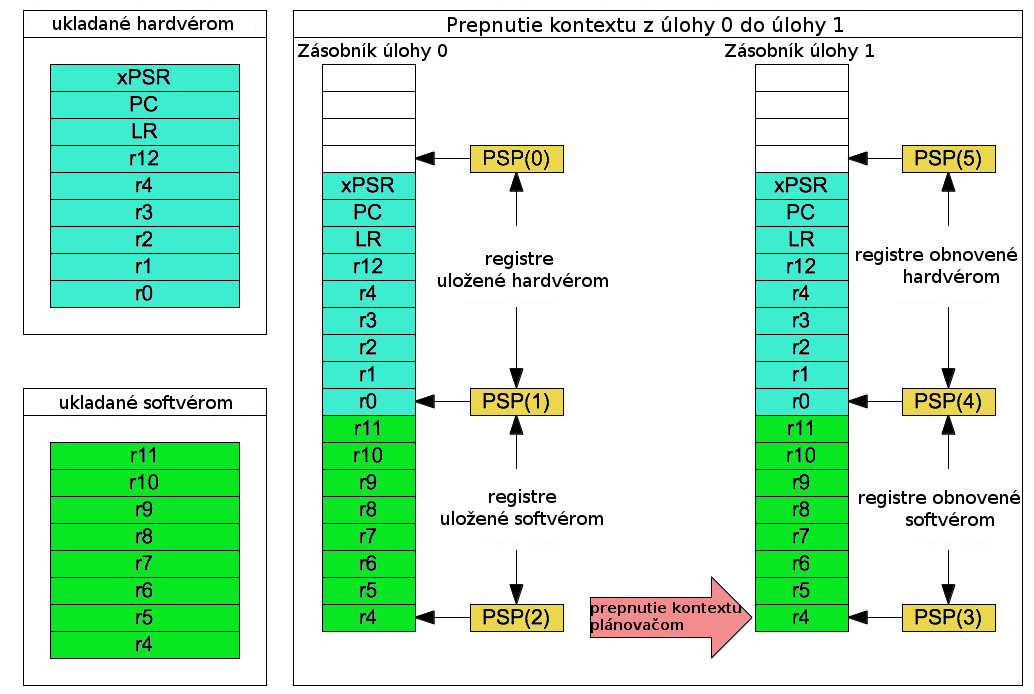
\includegraphics[width=.85\textwidth]{images/context_switch.png}
\caption{Prepnutie kontextu}
\label{obr2}
\end{center}
\end{minipage}
\end{center}
\end{figure}

Hardvér automaticky uloží registre R0..R5, R12, LR, PC a xPSR. V prípade jednoduchej obsluhy prerušenia to väčšinou postačuje a funkcia si vystačí s uvedenými registrami. V prípade prepnutia kontextu však nie je známe, či vlákna nevyužívajú aj zvyšné registre. Najmä pri rozsiahlejších funkciách kompilátor plne využije všetky registre. Nezostáva nič iné, ako uložiť všetky dostupné registre. Operácia je však veľmi rýchla a je realizovateľná jedinou inštrukciou :
{\small
\begin{verbatim}
__asm volatile("push {r4-r11}");
\end{verbatim}
}

Obnova kontextu je úplne analogická s ukladaním. Postupne sa vyberú registre, ktoré nie sú uložené hardvérom. Následne sa jadro informuje o tom, že sa vykonáva návrat z rutiny prerušenia, a že má vybrať aj zvyšné registre. Pokračujúca úloha bude teda opäť spustená bez zmeny registrov.
